%************************************************
\chapter{Neural Network Architectures for
EEG Decoding}\label{network-architectures}
%**************************************

\todotext{textbox}


We continued developing our neural network architectures with our
development strategy of progressing from networks that resemble
feature-based EEG decopding algorithms to more generic network
architectures. After the filterbank network from the master thesis, we
adapted the so-called shallow ConvNet, initally also developed in the
same master thesis \citep{schirrmeister_msc_thesis_2015}.
The shallow ConvNet still resembles filter bank common spatial patterns,
but less closely than the filterbank network. After validating that
these initial network architectures perform as well as filter bank
common spatial patterns, we progressed to developing and evaluating
substantially more generic architectures, namely the deep ConvNet and
the residual ConvNet.

In this section, I describe the architectures presented in our first
publication on EEG deep learning decoding
\citep{schirrmeisterdeephbm2017}. This part uses text and
figures from \citep{schirrmeisterdeephbm2017} adapted for
readibility in this thesis. The deep and residual ConvNet were primarily
developed by me together with help from my coauthors.


    \hypertarget{shallow-convnet-architecture}{%
\section{Shallow ConvNet
Architecture}\label{shallow-convnet-architecture}}

% 

\begin{figure}[ht]
    \myfloatalign
    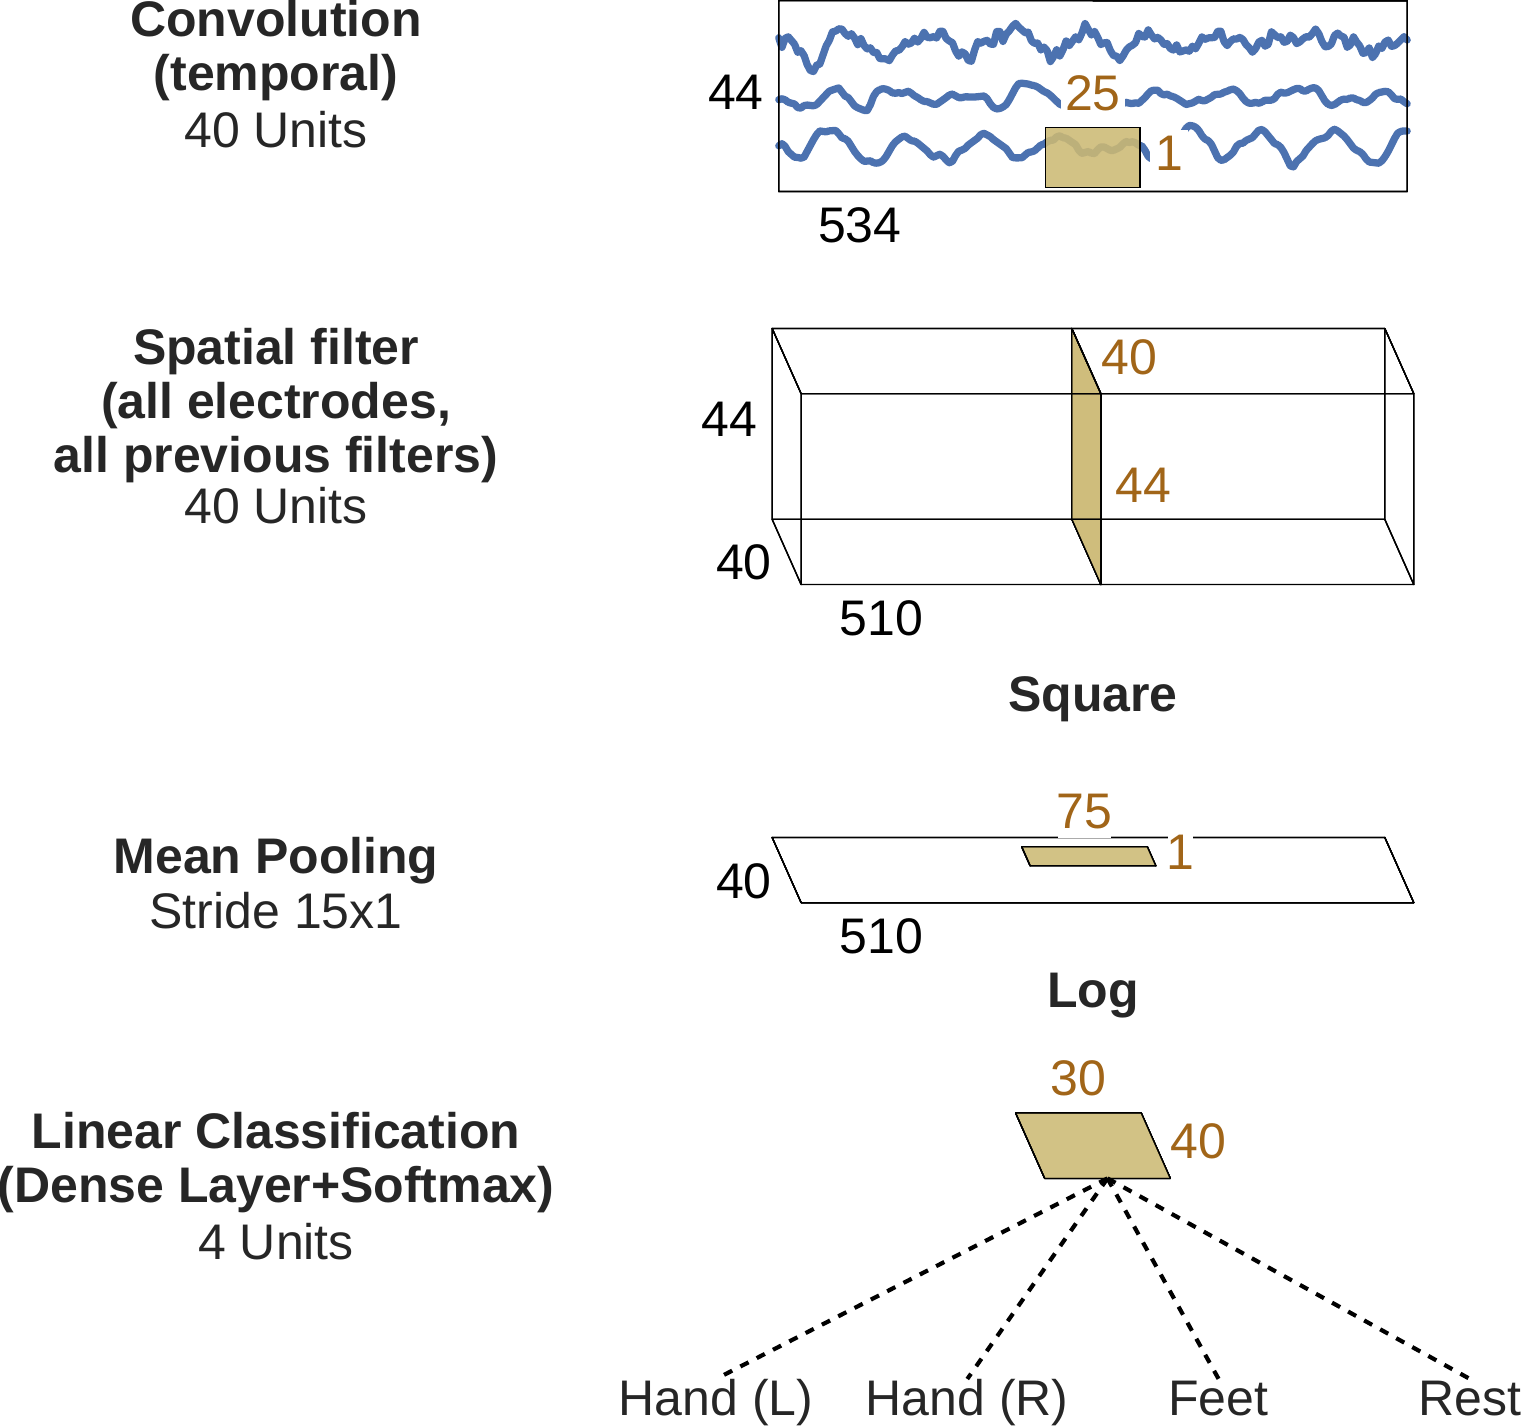
\includegraphics[width=0.8\linewidth]{images/3D_Diagram_MatplotLib.ipynb.0.png}
    \caption[Shallow ConvNet architecture]{
    \textbf{Shallow ConvNet architecture} EEG input (at the top) is
progressively transformed toward the bottom, until the final classifier
output. Black cuboids: inputs/feature maps; brown cuboids:
convolution/pooling kernels. The corresponding sizes are indicated in
black and brown, respectively. Note that the final dense layer operates
only on a small remaining temporal dimension, making it similar to a
regular convolutional layer. Figure from
\cite{schirrmeisterdeephbm2017}.}\label{shallow-net-figure}
\end{figure}



    We developed the shallow ConvNet architecture, a more flexible
architecture than the filterbank network that also learns temporal
filters on the input signal and on the later representation. Instead of
bandpass-filtered signals, it is fed the raw signals as input. The steps
the architecture implements are as follows (also see \Cref{shallow-net-figure}):

\begin{enumerate}
\item
\textbf{Temporal Filtering} Learnable temporal filters are indepedently convolved with the signals
of each EEG electrode. Afterwards, the channel dimension of the network
representation contains
\(\mathrm{electrodes} \cdot \mathrm{temporal~ filters}\) channels. 

\item
\textbf{Spatial Filtering} Combining spatial filtering with mixing the
outputs of the temporal filters, the network-channel dimension is
linearly transformed by learned weights to a smaller dimensionality for
further preprocessing. 

\item
\textbf{Log Average Power} The resulting feature timeseries are then squared, average-pooled and log-transformed, which allows the network to more easily learn log-power-based features. Unlike the filterbank network, the average pooling does not collapse the feature timeseries into one value per trial. So after these processing steps, still some temporal information about the timecourse of the variance throughout the trial can be preserved. 

\item
\textbf{Classifier} The final classification layer transforms these feature timecourses into class probabilities using a linear transformation and a softmax function.
\end{enumerate}


\section{Deep ConvNet Architecture}\label{deep-convnet-architecture}

\begin{figure}[ht]
    \myfloatalign
    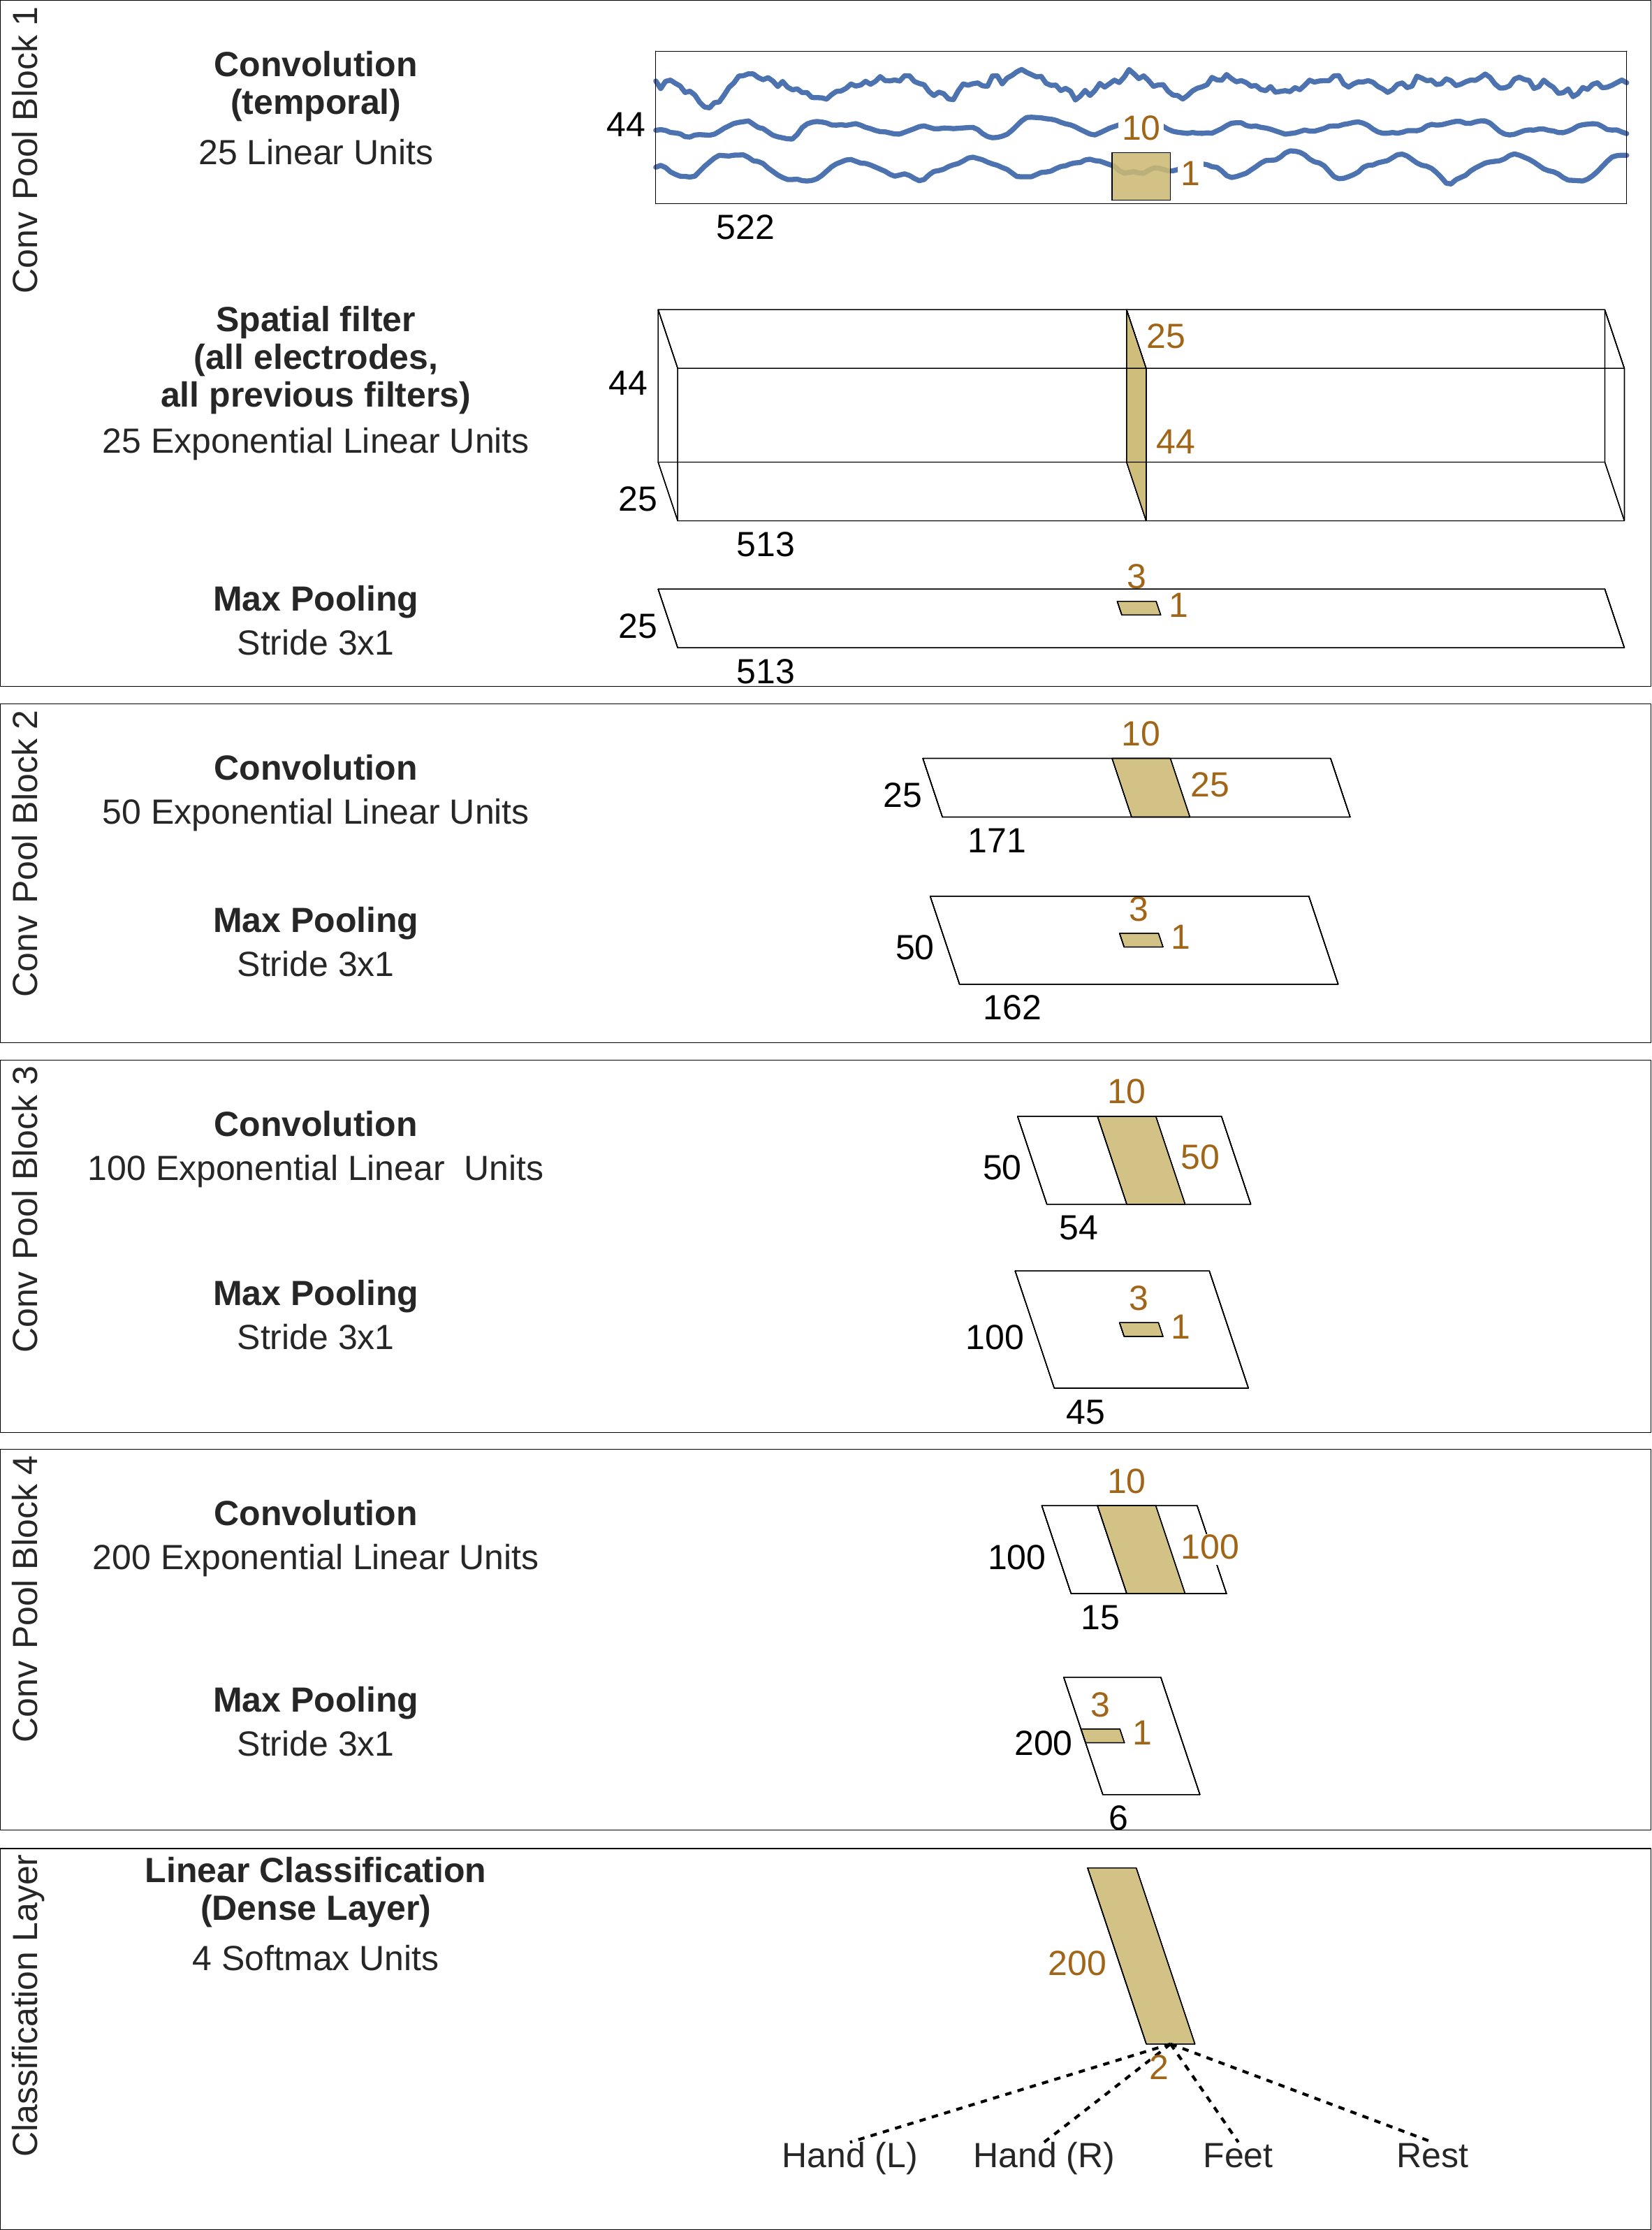
\includegraphics[width=0.9\linewidth]{images/3D_Diagram_MatplotLib.ipynb.1.png}
    \caption[Deep ConvNet architecture]{
    \textbf{Deep ConvNet architecture.}. Conventions as in \Cref{shallow-net-figure}. Figure from \citep{schirrmeisterdeephbm2017}}\label{deep-net-figure}
\end{figure}


    The deep ConvNet is a more generic architecture, closer to network
architectures used in computer vision, see
\Cref{deep-net-figure} for a schematic overview. The first
two temporal convolution and spatial filtering layers are the same in
the shallow network, which is followed by a ELU nonlinearity (ELUs, $f(x)=x$ for $x > 0$ and $f(x) = e^x-1$ for $x <= 0$) \cite{clevert_fast_2016}) and max pooling. The following
three blocks simply consist of a convolution, a ELU nonlinearity and a
max pooling. In the end, there is again a final linear classification
layer with a softmax function. Due to its less specific and more generic
computational steps, the deep architecture should be able to capture a
large variety of features. Hence, the learned features may also be less
biased towards the amplitude features commonly used in task-related EEG
decoding.


\section{Residual ConvNet
Architecture}\label{residual-convnet-architecture}


\begin{figure}[ht]
    \myfloatalign
    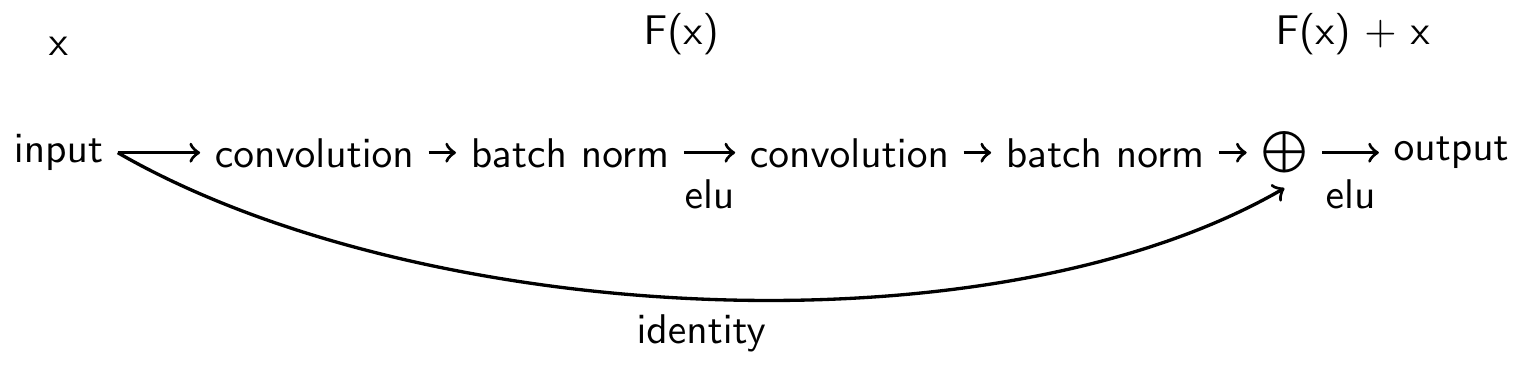
\includegraphics[width=1\linewidth]{images/residual_block.png}
    \caption[Residual block]{
    \textbf{Residual block.} Residual block used in the ResNet architecture
and as described in original paper (\citep{he_deep_2015}; see
Fig. 2) with identity shortcut option A, except using ELU instead of
ReLU nonlinearities. Figure from
\cite{schirrmeisterdeephbm2017}.}
\label{residual-net-figure}
\end{figure}

\begin{table}[ht]
    \small
    \myfloatalign
    \begin{tabularx}{\textwidth}{lS[table-format=3.0]ll} 
    \toprule
        \tableheadline{Layer/Block} & \tableheadline{\#Kernels}
        & \tableheadline{Kernel Size} & \tableheadline{ Output Size} \\ 
    \midrule
    Input & & & 1000x44x1 \\
    Convolution (linear) & 48 & 3x1 & 1000x44x48 \\
    Convolution (ELU) & 48 & 1x44 & 1000x1x48 \\
    ResBlock (ELU) & 48 & 3x1 & \\
    ResBlock (ELU) & 48 & 3x1 & \\
    ResBlock (ELU) & 96 & 3x1 (Stride 2x1) & 500x1x96 \\
    ResBlock (ELU) & 96 & 3x1 & \\
    ResBlock (ELU) & 144 & 3x1 (Stride 2x1) & 250x1x96 \\
    ResBlock (ELU) & 144 & 3x1 & \\
    ResBlock (ELU) & 144 & 3x1 (Stride 2x1) & 125x1x96 \\
    ResBlock (ELU) & 144 & 3x1 & \\
    ResBlock (ELU) & 144 & 3x1 (Stride 2x1) & 63x1x96 \\
    ResBlock (ELU) & 144 & 3x1 & \\
    ResBlock (ELU) & 144 & 3x1 (Stride 2x1) & 32x1x96 \\
    ResBlock (ELU) & 144 & 3x1 & \\
    ResBlock (ELU) & 144 & 3x1 (Stride 2x1) & 16x1x96 \\
    ResBlock (ELU) & 144 & 3x1 & \\
    Mean Pooling & & 10x1 & 7x1x144 \\
    Convolution + Softmax & 4 & 1x1 & 7x1x4 \\
        \bottomrule
    \end{tabularx}
    \caption[Residual ConvNet architecture hyperparameters.]{\textbf{Residual ConvNet architecture hyperparameters.}
Number of kernels, kernel and output size for all subparts of the
network. Output size is always time x height x channels. Assuming four output classes. Note that
channels here refers to input channels of a network layer, not to EEG
channels; EEG channels are in the height dimension. Output size is only
shown if it changes from the previous block. Second convolution and all
residual blocks used ELU nonlinearities. Note that in the end we had
seven outputs, i.e., predictions for the four classes, in the time
dimension (\textbf{7}x1x4 final output size). In practice, when using
cropped training as explained in the following chapter, we even had 424
predictions, and used the mean of these to predict the trial.}  
\label{residual-architectures-table}
\end{table}

    We also developed a residual ConvNet (\citep{he_deep_2015})
for EEG decoding. Residual networks add the input of a residual
computational block back to its output, and this allows to stably train
much deeper networks. We use the same residual blocks as the original
paper, described in Figure \Cref{residual-net-figure}. Our
residual ConvNet used ELU activation functions throughout the network
(same as the deep ConvNet) and also starts with a splitted temporal and
spatial convolution (same as the deep and shallow ConvNets), followed by
14 residual blocks, mean pooling and a final softmax dense
classification layer.

In total, the residual ConvNet has 31 convolutional layers, a depth
where ConvNets without residual blocks started to show problems
converging in the original residual networks paper
\citep{he_deep_2015}. In layers where the number of channels
is increased, we padded the incoming feature map with zeros to match the
new channel dimensionality for the shortcut, as in option A of the
original paper \citep{he_deep_2015}. The overall architecture is also shown in
\Cref{residual-architectures-table}.

\todotext{textbox}
